
\documentclass[11pt]{asaproc}\usepackage[]{graphicx}\usepackage[]{color}
%% maxwidth is the original width if it is less than linewidth
%% otherwise use linewidth (to make sure the graphics do not exceed the margin)
\makeatletter
\def\maxwidth{ %
  \ifdim\Gin@nat@width>\linewidth
    \linewidth
  \else
    \Gin@nat@width
  \fi
}
\makeatother

\definecolor{fgcolor}{rgb}{0.345, 0.345, 0.345}
\newcommand{\hlnum}[1]{\textcolor[rgb]{0.686,0.059,0.569}{#1}}%
\newcommand{\hlstr}[1]{\textcolor[rgb]{0.192,0.494,0.8}{#1}}%
\newcommand{\hlcom}[1]{\textcolor[rgb]{0.678,0.584,0.686}{\textit{#1}}}%
\newcommand{\hlopt}[1]{\textcolor[rgb]{0,0,0}{#1}}%
\newcommand{\hlstd}[1]{\textcolor[rgb]{0.345,0.345,0.345}{#1}}%
\newcommand{\hlkwa}[1]{\textcolor[rgb]{0.161,0.373,0.58}{\textbf{#1}}}%
\newcommand{\hlkwb}[1]{\textcolor[rgb]{0.69,0.353,0.396}{#1}}%
\newcommand{\hlkwc}[1]{\textcolor[rgb]{0.333,0.667,0.333}{#1}}%
\newcommand{\hlkwd}[1]{\textcolor[rgb]{0.737,0.353,0.396}{\textbf{#1}}}%
\let\hlipl\hlkwb

\usepackage{framed}
\makeatletter
\newenvironment{kframe}{%
 \def\at@end@of@kframe{}%
 \ifinner\ifhmode%
  \def\at@end@of@kframe{\end{minipage}}%
  \begin{minipage}{\columnwidth}%
 \fi\fi%
 \def\FrameCommand##1{\hskip\@totalleftmargin \hskip-\fboxsep
 \colorbox{shadecolor}{##1}\hskip-\fboxsep
     % There is no \\@totalrightmargin, so:
     \hskip-\linewidth \hskip-\@totalleftmargin \hskip\columnwidth}%
 \MakeFramed {\advance\hsize-\width
   \@totalleftmargin\z@ \linewidth\hsize
   \@setminipage}}%
 {\par\unskip\endMakeFramed%
 \at@end@of@kframe}
\makeatother

\definecolor{shadecolor}{rgb}{.97, .97, .97}
\definecolor{messagecolor}{rgb}{0, 0, 0}
\definecolor{warningcolor}{rgb}{1, 0, 1}
\definecolor{errorcolor}{rgb}{1, 0, 0}
\newenvironment{knitrout}{}{} % an empty environment to be redefined in TeX

\usepackage{alltt}

\usepackage{graphicx}
\usepackage{natbib}
\usepackage[hyphens]{url}
\usepackage{color}
\usepackage{times}
\usepackage{verbatim}
%\usepackage{enumitem}
\usepackage[hidelinks,breaklinks=true]{hyperref}


\renewcommand\labelenumi{(\roman{enumi})}
\renewcommand\theenumi\labelenumi

\title{An Interactive Tool to Visualize Results from Uncertainty Quantification}

\author{Matthew Isaac \thanks{Department of Mathematics and Statistics, Utah State University, Logan, UT 84322--3900, USA. 
E-mail: \url{matt.isaac@aggiemail.usu.edu}}
}
\IfFileExists{upquote.sty}{\usepackage{upquote}}{}
\begin{document}

\renewcommand{\topfraction}{1.0}
\renewcommand{\bottomfraction}{1.0}
\renewcommand{\textfraction}{0.0}
\renewcommand{\floatpagefraction}{1.0}
\renewcommand{\dbltopfraction}{1.0}


\maketitle

\begin{abstract}
Uncertainty quantification is a class of methods used to simulate the ways that variations to inputs of a system can potentially change the end state of that system. This article outlines the implementation of an interactive tool to visualize the results of an uncertainty quantification analysis. The interactive tool is a deployable web application built with the {\tt R Shiny} framework. Users can create, adjust, and save custom visualizations to assist in interpreting and presenting results. 
\end{abstract}

\begin{keywords} Interactive Visualization; {\tt shiny} R Package
\end{keywords}


%%%%%%%%%%%%%%%%%%%%%%%%%
\section{Introduction}
\label{Introduction}
%%%%%%%%%%%%%%%%%%%%%%%%%

Uncertainty quantification is a methodological framework used with some frequency in engineering analysis \citep{EW2018}. It is used to understand how variability  within the parameters (i.e. inputs) to some system impact the end state of that system. Engineering analysts use uncertainty quantification to assess and find the balance between design sufficiency and design efficiency. This is particularly important in fields where large-scale prototypes, testing, and data collection are extremely expensive. Engineers in these types of applications are increasingly relying on computational simulations to assess system designs.

In the following article, I outline the implementation of an interactive tool to visualize uncertainty quantification results. The outline of this article will proceed as follows: In Section~\ref{UQOverview}, a brief overview of uncertainty quantification is given. In Section~\ref{Methods}, the methods by which the visualization tool was developed are described. In Section~\ref{Results}, features of the resulting web application is described. In Section~\ref{Discussion}, challenges with and future enhancements to the web application are discussed. The code written to generate the {\tt shiny} app is included in the Appendix.

%%%%%%%%%%%%%%%%%%%%%%%%%
\section{Uncertainty Quantification Overview}  
\label{UQOverview}
%%%%%%%%%%%%%%%%%%%%%%%%%

The following description of the uncertainty quantification algorithm is adapted from \cite{EW2018}. First, a few terms and definitions will be described. 

\begin{description}
\item[system response quantity (SRQ):] A parameter of particular interest directly related to the engineering system in question. The SRQ is the output (i.e. prediction) from the engineering model.
\item[engineering model:] A mathematical model that defines the relationship between the parameters (model inputs) and SRQ (model output). 
\item[aleatory uncertainty:] Uncertainty resulting from randomness inherent to a given parameter. Gaining more knowledge about the parameter will not reduce the uncertainty of the parameter. 
\item[epistemic uncertainty:] Uncertainty resulting from a lack of knowledge about a given parameter. Gaining more knowledge about the parameter could reduce the uncertainty of the parameter. 
\end{description}

The first step of uncertainty quantification is to identify sources of uncertainty (model parameters) and classify them as either aleatory or epistemic. This classification process has been somewhate debated in literature \citep{KD2009}, and will not be discussed as it is outside the scope of this project. Once these uncertainties related to the model parameters have been identified and classified as aleatory or epistemic, the uncertainty for each parameter must somehow be described. Traditionally, epistemic uncertainties have been described by an interval over which any value in the interval is equally likely, while aleatory uncertainties have been assigned probability distributions. Some more recent publications \citep{EW2018} propose that all uncertainties, aleatory or epistemic, be described using probability distributions. This debate will not be discussed here as it is, again, outside the scope of this project. Once these distributions and/or intervals have all been assigned, they are carried through the model using Monte Carlo techniques.

Let $m$ denote the number of iterations of an outer for loop, and let $n$ denote the number of iterations in an inner for loop. In the outer for loop, values for the epistemic uncertainty parameters are selected randomly from the intervals/distributions assigned. Upon entering the inner loop, values for the aleatory uncertainty parameters are randomly chosen from the distributions assigned. The values chosen for the parameters in both the outer loop and the inner loop are then used as inputs in the engineering model to calculate a value for the SRQ. This value is stored and the inner loop continues running for the rest of the $n-1$ iterations. All of the $n$ SRQ values calculated from the $n$ iterations of the inner loop are used to calculate an empirical cumulative distribution function (CDF) of SRQ values and the CDF is stored. The outer loop then begins its second iteration, and new values for the empirical uncertainty parameters are chosen. The inner loop then runs another $n$ iterations, producing another CDF. This process continues until the outer loop has run all of its $m$ iterations. 

At this point, there will be $m$ empirical CDFs that have been calculated, representing various possible realized values of the SRQ. These CDFs can then be plotted and interpreted. \cite{EW2018} suggests constructing a ``P-box". This P-box is found by calculating a lower percentile (e.g. the 5th percentile) and an upper percentile (e.g. the 95th percentile) of the CDF ensemble. This P-box can then be interpreted in several ways, including (1) selecting a SRQ value and extracting a probability interval, and (2) selecting a probability value and extracting an SRQ interval.

%%%%%%%%%%%%%%%%%%%%%%%%%
\section{Methods}  
\label{Methods}
%%%%%%%%%%%%%%%%%%%%%%%%%

In order to assist analysts in visualizing and interpreting results from an uncertainty quantification analysis as described in Section~\ref{UQOverview}, an interactive visualization tool was developed. Since the actual uncertainty quantification analysis can be carried out with greater speed and computational power elsewhere, this implementation does not include the Monte Carlo portion of the algorithm described in Section~\ref{UQOverview}. The web application was built using the {\tt shiny R} package \citep{SHINY} and the code for this application is contained in two files. The first file, {\tt ui.R} (short for `user interface') contains the code that controls the layout of the various panels and panes in the application, as well as the placement of the user interface elements (i.e. text inputs, sliders, etc.). The {\tt server.R} file contains the computational code that performs calculations, data manipulation, and generates the plots. The source code is included in the Appendix.

\subsection{{\tt R} Packages}
The following software packages were used in the development of the web application:

\begin{description}

\item[{\bf R:}] The code for the web application was written in the {\tt R} programming language \citep{R}.

\item[{\bf RStudio:}] Rstudio \citep{RSTUDIO} is an integrated development environment that was used to both develop and deploy the web application.

\item[{\bf shiny:}] The {\tt shiny} package and framework \citep{SHINY} constitues the backbone of this project. {\tt shiny} provides a way to create and deploy web applications through RStudio \citep{RSTUDIO}. It also contains the implementations for all user-interface components (toggle buttons, check boxes, numeric inputs, sliders, etc.). The {\tt shinydashboard} package \citep{DASH} was also used as an aesthetic wrapper around the {\tt shiny} framework. The {\tt shiny} package was be used to create and will be used to deploy the web application.

\item[{\bf ggplot2:}] The plotting functionality of the {\tt ggplot2} package \citep{GGPLOT} was used to generate the actual visualization and to add, remove, or adjust components on the plot. 

\item[{\bf shinydashboard:}] The {\tt shinydashboard} package \citep{DASH} was used as an aesthetic wrapper to the web application to improve its professional appearance. 

\item[{\bf shinyalert:}] The {\tt shinyalert} package \citep{SALERT} was used to create a pop-up message when the user takes certain actions.

\item[{\bf shinyWidgets:}] The {\tt shinyWidgets} package \citep{SWIDGET} was used to create custom toggle buttons.

\end{description}

\vspace{5mm}

Since the existing {\tt R} packages already implemented most of the tools needed to generate the plot and implement user interface elements, the primary task on this project was to seamlessly combine elements from the packages above (particularly the {\tt shiny}, {\tt ggplot2} packages) to create a user-friendly interactive visualization tool. 

%%%%%%%%%%%%%%%%%%%%%%%%%
\section{Results}
\label{Results}
%%%%%%%%%%%%%%%%%%%%%%%%%

The resulting web application currently several main features implemented. The web application is currently deployed at \url{https://misaac.shinyapps.io/UQViz/}. The following subsections outlines the basic functionality. 

\subsection{Data Source}
The `Data Source' tab contains the controls that allow the user to select either a sample data set (provided for convenience) or to upload their own {\tt .csv} file. If data from a file is to be used, the x-values over which the CDFs are evaluated should be the first column, and the CDF y-values in the following columns. 

\subsection{Visualization Options}
Several visualization options are provided to allow customizable graphics to be created. The `Show/Hide P-box' and the `Show/Hide CDFs' buttons toggle back and forth between showing and hiding the red P-box and the black ensemble of CDFs. Note that showing the CDF ensemble may (depending on the size of the uploaded file) significantly increase plot rendering times.

The P-box lower and upper percentiles default to 0.05 and 0.95. Users can modify this by inputting the desired lower and upper percentile to be used in the visualization. 

Moving the `CDF Transparency' slider will make each individual CDF trace more or less transparent. A slider value of 1 corresponds to completely opaque, while a slider value of 0 corresponds to completely transparent. This mitigates the issue of overplotting that can often arise when hundreds or thousands traces are shown on the same plot. Allowing for some transparency allows the user to visualize the density of regions within the CDF ensemble. Figure~\ref{viz_opt} shows plots with several possible visualization options selected. A screenshot of the visualization option control panel is shown in Figure~\ref{tab_vo}.

\begin{figure}[t]
\begin{center} 
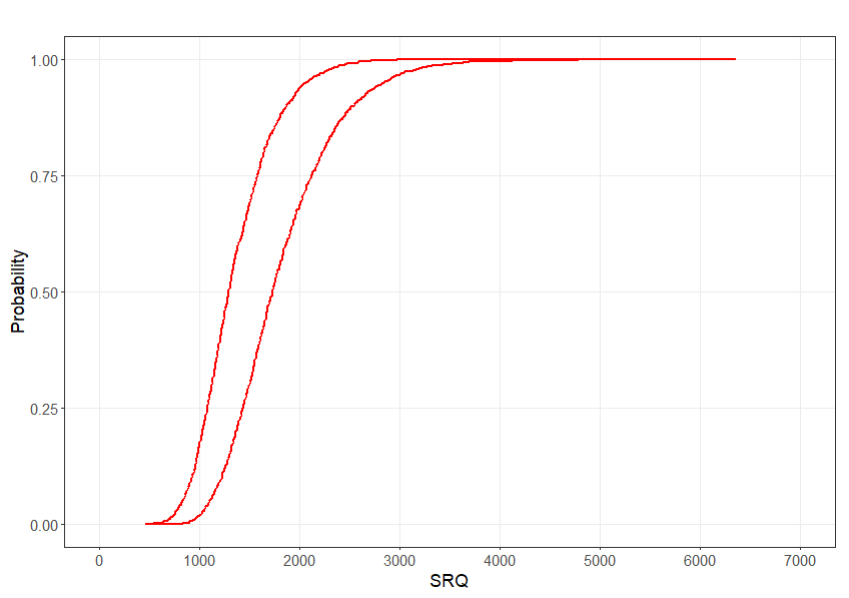
\includegraphics[height=4.2cm,width=4.5cm]{figures2/pbx_only.png}
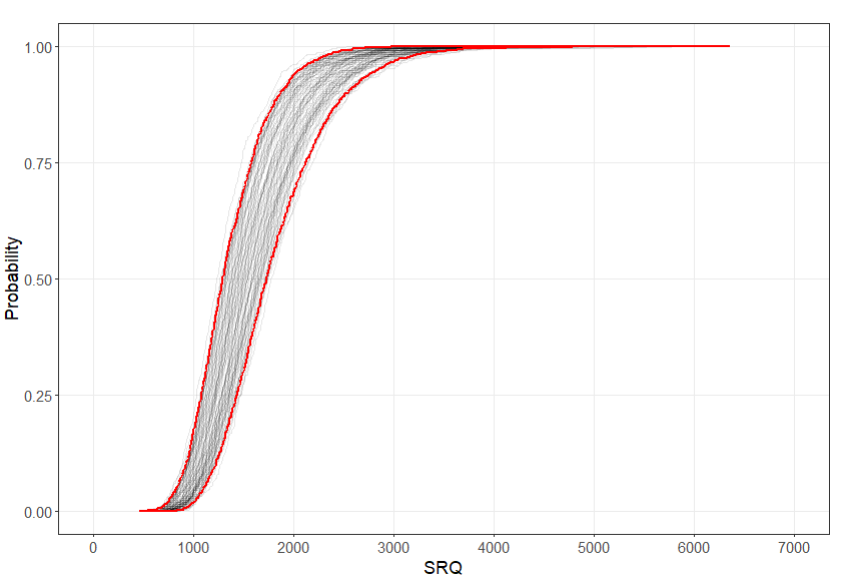
\includegraphics[height=4.1cm,width=4.5cm]{figures2/pbx_cdf_d.png}
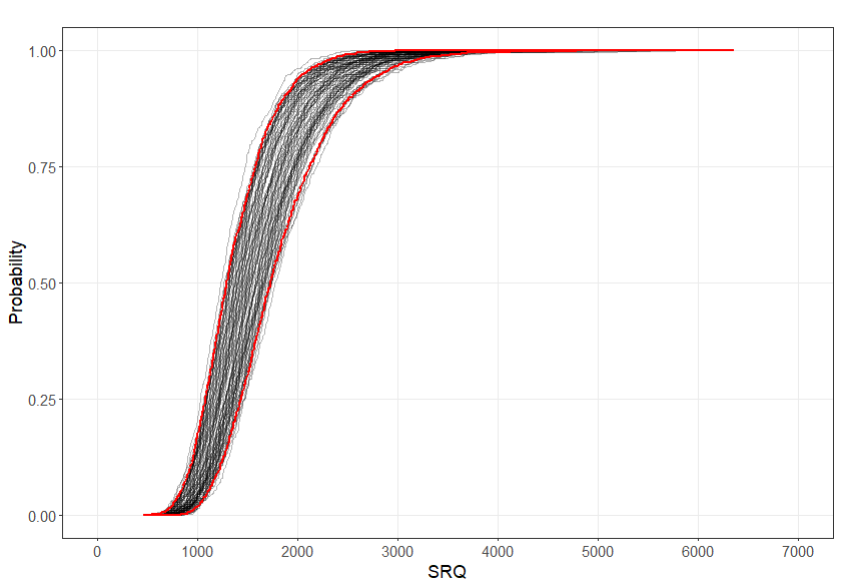
\includegraphics[height=4.1cm,width=4.5cm]{figures2/pbx_cdf_l.png} 
\end{center} 
\caption{\label{viz_opt}Visualization with P-box shown and CDfs hidden (left); Visualization with P-box and CDFs both shown with high transparency (center) and low transparency (right)}
\end{figure}


\begin{figure}[t]
\begin{center} 
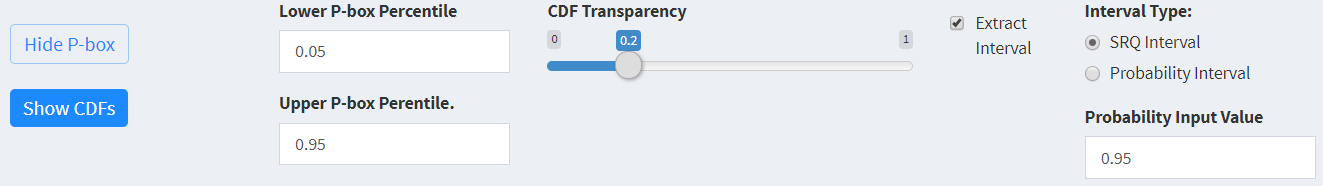
\includegraphics[height=2cm,width=14cm]{figures2/tab_vo.png}
\end{center} 
\caption{\label{tab_vo}Screenshot from the web application of visualization option control panel}
\end{figure}

To aid with interpretation, both probability intervals and SRQ intervals can be extracted from the P-box shown in the visualization, as described in \cite{EW2018}. To extract a probability interval, the user selects an SRQ value at which a line is drawn vertically. The intersections of the vertical line with the P-box create the lower and upper endpoints for the probability interval. In a similar process, the user can also extract a SRQ interval by selecting a probability value at which a line is drawn horizontally. The intersections of the horizontal line with the P-box create the SRQ interval. This process is illustrated in Figure~\ref{ext_int}. 

\begin{figure}[t]
\begin{center}
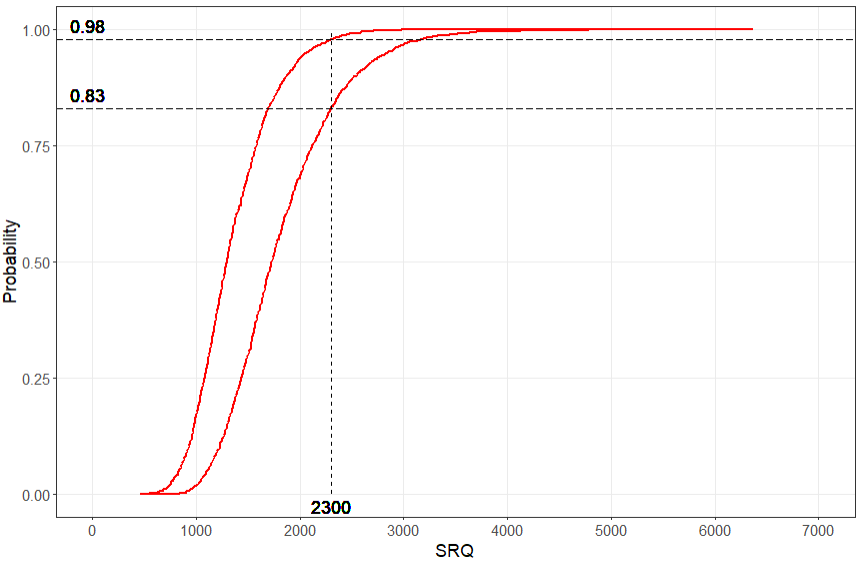
\includegraphics[height=5cm,width=6cm]{figures2/prob_int.png}
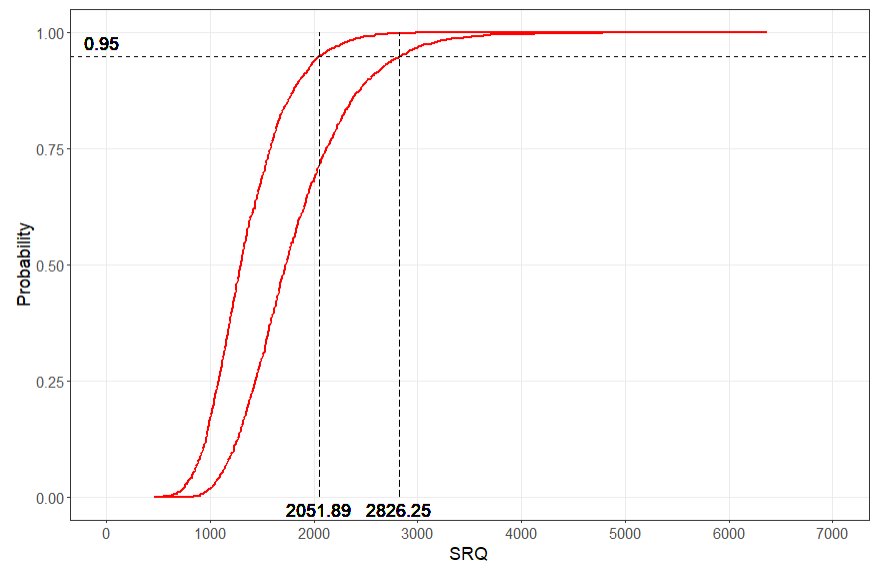
\includegraphics[height=5cm,width=6.5cm]{figures2/srq_int.png}
\end{center}
\caption{\label{ext_int}Extracting a probability interval (left); Extracting an SRQ interval (right)}
\end{figure}

A title and can be added to the plot and the x-axis label can be changed from the default label of `SRQ'. This allows users to futher customize the visualization to a specific domain or context. 

Users can download and save a {\tt .png} version of the current rendering of the visualization by providing a file name and clicking the `Download' button. 



%%%%%%%%%%%%%%%%%%%%%%%%%
\section{Discussion}
\label{Discussion}
%%%%%%%%%%%%%%%%%%%%%%%%%

\subsection{Challenges}
One main challenge with this visualization tool is the time that it would takes to render the plot when the CDF ensemble is shown. The nature of uncertainty quantificataion and this kind of visualization leads to there being hundreds or even thousands of traces on a single plot. In addition, the way the interactive features are implemented through the {\tt shiny} package causes the plot to completely re-render when user inputs change. Thus, whenever the user selects a new plotting option and the CDFs are currently shown, he or she must wait several seconds (depending on the size of the data set being used) for the plot to re-render. This leads to a less `interactive' feel for the user. No immediate or direct solution has been found for this issue yet. However, an effective workaround, as described the the User Guide tab on the web application, has been suggested. If the user wishes to display the CDF ensemble on the final version of the plot, it is suggested to adjust all visualization options and controls while the CDFs are hidden, keeping the plot rendering times to a reasonable length. Then, as the last step, show the CDF ensemble. This way, the user will only have to wait once for the long rendering time.

\subsection{Future Work}
Further work in developing this visualization tool may involve researching other methods for visualizing uncertainty, such as the methods described in \cite{JA2008}, and implementing several methods for visualization. This would allow users to choose from various visualization methods within the web application to create a graphic that is best suited to a given context. Another extension of this visualization tool could be to use it in a self contained UQ tool, where users could perform the entire UQ algorithm from start to finish. For example, users could define the engineering model to be used, define parameters as aleatory or epistemic, carry out the UQ algorithm, and visualize the results. However, as the web application now stands, it can be used to assist engineers and analysts in visualizing, understanding, and interpreting results from uncertainty quantification analyses. 


\newpage

\bibliographystyle{elsarticle-harv}
% modified to add 
%     \itemsep=0pt
% to 2nd line of file paper.bbl
\bibliography{references2}

\newpage
%%%%%%%%%%%%%%%%%%%%%%%%%
\appendix
\section{Appendix}
\label{Appendix}
%%%%%%%%%%%%%%%%%%%%%%%%%

% {\tt R} code for {\tt shiny} web application.

\subsection{Source Code: {\tt ui.R}}

{\scriptsize
\begin{knitrout}
\definecolor{shadecolor}{rgb}{0.969, 0.969, 0.969}\color{fgcolor}\begin{kframe}
\begin{alltt}
\hlkwd{library}\hlstd{(shiny)}
\hlkwd{library}\hlstd{(shinydashboard)}
\hlkwd{library}\hlstd{(plotly)}
\hlkwd{library}\hlstd{(shinyalert)}
\hlkwd{library}\hlstd{(shinyWidgets)}

\hlstd{cranURL} \hlkwb{<-} \hlstr{"https://cran.r-project.org/web/packages/"}

\hlkwd{dashboardPage}\hlstd{(}
  \hlkwd{dashboardHeader}\hlstd{(}
    \hlkwc{title} \hlstd{=} \hlstr{"UQViz"}
  \hlstd{),}
  \hlkwd{dashboardSidebar}\hlstd{(}
  \hlstd{),}
  \hlkwd{dashboardBody}\hlstd{(}
    \hlkwd{useShinyalert}\hlstd{(),}
    \hlkwd{tabsetPanel}\hlstd{(}
      \hlkwd{tabPanel}\hlstd{(}\hlstr{"Data Source"}\hlstd{,}
               \hlkwd{fluidRow}\hlstd{(}
                 \hlkwd{column}\hlstd{(}
                   \hlkwc{width} \hlstd{=} \hlnum{3}\hlstd{,}
                   \hlkwd{radioButtons}\hlstd{(}\hlkwc{inputId} \hlstd{=} \hlstr{"radioDataSource"}\hlstd{,}
                                \hlkwc{label} \hlstd{=} \hlstr{"Data Source"}\hlstd{,}
                                \hlkwc{choices} \hlstd{=} \hlkwd{c}\hlstd{(}\hlstr{"Sample Data"}\hlstd{,}
                                            \hlstr{"File Upload"}\hlstd{),}
                                \hlkwc{selected} \hlstd{=} \hlstr{"Sample Data"}\hlstd{),}
                   \hlkwd{uiOutput}\hlstd{(}\hlkwc{outputId} \hlstd{=} \hlstr{"fileInput"}\hlstd{)}
                 \hlstd{)}
               \hlstd{)}

      \hlstd{),}
      \hlkwd{tabPanel}\hlstd{(}\hlstr{"Visualization Options"}\hlstd{,}
               \hlkwd{fluidRow}\hlstd{(}
                 \hlkwd{column}\hlstd{(}
                   \hlkwc{width} \hlstd{=} \hlnum{2}\hlstd{,}
                   \hlkwc{offset} \hlstd{=} \hlnum{0}\hlstd{,}
                   \hlkwd{verticalLayout}\hlstd{(}
                     \hlkwd{br}\hlstd{(),}
                     \hlkwd{uiOutput}\hlstd{(}\hlkwc{outputId} \hlstd{=} \hlstr{"pbxBttn"}\hlstd{),}
                     \hlkwd{br}\hlstd{(),}
                     \hlkwd{uiOutput}\hlstd{(}\hlkwc{outputId} \hlstd{=} \hlstr{"cdfBttn"}\hlstd{)}

                   \hlstd{)}

                 \hlstd{),}
                 \hlkwd{column}\hlstd{(}
                   \hlkwc{width} \hlstd{=} \hlnum{2}\hlstd{,}
                   \hlkwc{offset} \hlstd{=} \hlnum{0}\hlstd{,}
                   \hlkwd{numericInput}\hlstd{(}\hlkwc{inputId} \hlstd{=} \hlstr{"pboxLower"}\hlstd{,}
                                \hlkwc{label} \hlstd{=} \hlstr{"Lower P-box Percentile"}\hlstd{,}
                                \hlkwc{value} \hlstd{=} \hlnum{0.05}\hlstd{,}
                                \hlkwc{width} \hlstd{=} \hlnum{250}\hlstd{),}
                   \hlkwd{numericInput}\hlstd{(}\hlkwc{inputId} \hlstd{=} \hlstr{"pboxUpper"}\hlstd{,}
                                \hlkwc{label} \hlstd{=} \hlstr{"Upper P-box Perentile."}\hlstd{,}
                                \hlkwc{value} \hlstd{=} \hlnum{0.95}\hlstd{,}
                                \hlkwc{width} \hlstd{=} \hlnum{250}\hlstd{)}
                 \hlstd{),}
                 \hlkwd{column}\hlstd{(}
                   \hlkwc{width} \hlstd{=} \hlnum{3}\hlstd{,}
                   \hlkwc{offset} \hlstd{=} \hlnum{0}\hlstd{,}
                   \hlkwd{sliderInput}\hlstd{(}\hlkwc{inputId} \hlstd{=} \hlstr{"sliderAlpha"}\hlstd{,}
                               \hlkwc{label} \hlstd{=} \hlstr{"CDF Transparency"}\hlstd{,}
                               \hlkwc{value} \hlstd{=} \hlnum{0.2}\hlstd{,}
                               \hlkwc{min} \hlstd{=} \hlnum{0}\hlstd{,}
                               \hlkwc{max} \hlstd{=} \hlnum{1}\hlstd{,}
                               \hlkwc{step} \hlstd{=} \hlnum{0.1}\hlstd{,}
                               \hlkwc{ticks} \hlstd{=} \hlnum{FALSE}\hlstd{)}
                 \hlstd{),}
                 \hlkwd{column}\hlstd{(}
                   \hlkwc{width} \hlstd{=} \hlnum{1}\hlstd{,}
                   \hlkwc{offset} \hlstd{=} \hlnum{0}\hlstd{,}
                   \hlkwd{checkboxInput}\hlstd{(}\hlkwc{inputId} \hlstd{=} \hlstr{"extractInt"}\hlstd{,}
                                 \hlkwc{label} \hlstd{=} \hlstr{"Extract Interval"}\hlstd{,}
                                 \hlkwc{value} \hlstd{=} \hlnum{FALSE}\hlstd{)}

                 \hlstd{),}
                 \hlkwd{column}\hlstd{(}
                   \hlkwc{width} \hlstd{=} \hlnum{2}\hlstd{,}
                   \hlkwd{uiOutput}\hlstd{(}\hlkwc{outputId} \hlstd{=} \hlstr{"extractTypeInput"}\hlstd{),}
                   \hlkwd{uiOutput}\hlstd{(}\hlkwc{outputId} \hlstd{=} \hlstr{"valInput"}\hlstd{)}
                 \hlstd{)}
               \hlstd{)}

      \hlstd{),}
      \hlkwd{tabPanel}\hlstd{(}\hlstr{"Labeling"}\hlstd{,}
               \hlkwd{fluidRow}\hlstd{(}
                 \hlkwd{column}\hlstd{(}
                   \hlkwc{width} \hlstd{=} \hlnum{2}\hlstd{,}
                   \hlkwd{textInput}\hlstd{(}\hlkwc{inputId} \hlstd{=} \hlstr{"titleInput"}\hlstd{,}
                             \hlkwc{label} \hlstd{=} \hlstr{"Title"}\hlstd{,}
                             \hlkwc{placeholder} \hlstd{=} \hlstr{"Plot Title"}\hlstd{,}
                             \hlkwc{value} \hlstd{=} \hlstr{""}\hlstd{)}
                 \hlstd{),}
                 \hlkwd{column}\hlstd{(}
                   \hlkwc{width} \hlstd{=} \hlnum{2}\hlstd{,}
                   \hlkwd{textInput}\hlstd{(}\hlkwc{inputId} \hlstd{=} \hlstr{"xaxisInput"}\hlstd{,}
                             \hlkwc{label} \hlstd{=} \hlstr{"X axis Label"}\hlstd{,}
                             \hlkwc{placeholder} \hlstd{=} \hlstr{"X-axis"}\hlstd{,}
                             \hlkwc{value} \hlstd{=} \hlstr{"SRQ"}\hlstd{)} \hlcom{#,}
                   \hlcom{# textInput(inputId = "yaxisInput", }
                   \hlcom{#           label = "Y axis Label", }
                   \hlcom{#           placeholder = "Y-axis", }
                   \hlcom{#           value = "Probability")}
                 \hlstd{)}
               \hlstd{)),}
      \hlkwd{tabPanel}\hlstd{(}\hlstr{"User Guide"}\hlstd{,}
               \hlkwd{h3}\hlstd{(}\hlstr{"Overview"}\hlstd{),}
               \hlkwd{h5}\hlstd{(}\hlstr{"UQViz is an interactive tool that can be used 
                  to create meaningful visualizations of
                  '2D Uncertainty Quantification' 
                  (for more information on 2D UQ, see "}\hlstd{,}
                  \hlstd{tags}\hlopt{$}\hlkwd{a}\hlstd{(}
                    \hlkwc{href} \hlstd{=} \hlkwd{paste0}\hlstd{(}\hlstr{"http://verification.asmedigitalcollection"}\hlstd{,}
                                  \hlstr{".asme.org"}\hlstd{,}
                                  \hlstr{"/article.aspx?articleid="}\hlstd{,}
                                  \hlstr{"2703289&resultClick=1"}\hlstd{),}
                         \hlstr{"this article"}\hlstd{,}
                         \hlkwc{target} \hlstd{=} \hlstr{"_blank"}\hlstd{),}
                  \hlstr{"). Users can select data source and adjust various 
                  visual components and labels. The title and axis
                  label can also be customized, and the visualization 
                  can be downloaded and saved."}\hlstd{),}
               \hlkwd{h3}\hlstd{(}\hlstr{"Data Source"}\hlstd{),}
               \hlstd{tags}\hlopt{$}\hlkwd{p}\hlstd{(}\hlstr{"The 'Data Source' tab contains controls for 
                      the user to select the source from 
                      which data for the visualization will be obtained.
                      If "}\hlstd{,}
                      \hlstd{tags}\hlopt{$}\hlkwd{b}\hlstd{(}\hlstr{'Sample Data'}\hlstd{),}
                      \hlstr{"is selected, a small built-in data set is used as 
                      the data source for the 
                      visualization. This feature is provided for convenience, 
                      and can be used for experimentation and 
                      exploration. If "}\hlstd{,}
                      \hlstd{tags}\hlopt{$}\hlkwd{b}\hlstd{(}\hlstr{'File Upload'}\hlstd{),} \hlstr{"
                      is selected, users can upload a "}\hlstd{,}
                      \hlstd{tags}\hlopt{$}\hlkwd{code}\hlstd{(}\hlstr{".csv"}\hlstd{),}
                      \hlstr{"file containing
                      data to be used in the visualization. This "}\hlstd{,}
                      \hlstd{tags}\hlopt{$}\hlkwd{code}\hlstd{(}\hlstr{".csv"}\hlstd{),}
                      \hlstr{"file should be formatted such that the 'x' values over 
                      which the CDFs are evaluated 
                      are in the first column, and the CDFs are 
                      in the following columns."}
               \hlstd{),}
               \hlkwd{h3}\hlstd{(}\hlstr{"Visualization Options"}\hlstd{),}
               \hlstd{tags}\hlopt{$}\hlkwd{p}\hlstd{(}\hlstr{"Several visualization options are provided to
                      allow customizable graphics to be
                      created. The "}\hlstd{,}
                      \hlstd{tags}\hlopt{$}\hlkwd{b}\hlstd{(}\hlstr{"Show/Hide P-box"}\hlstd{),} \hlstr{" and the "}\hlstd{,}
                      \hlstd{tags}\hlopt{$}\hlkwd{b}\hlstd{(}\hlstr{"Show/Hide CDFs"}\hlstd{),} \hlstr{" buttons toggle
                      back and forth between showing and 
                      hiding the red P-box and the black ensemble of CDFs. 
                      Note that showing the CDF 
                      ensemble may (depending on the size of the uploaded
                      file) significantly increase
                      plot rendering times. If the user wishes to
                      display the CDFs on the final version
                      of the plot, it is suggested to adjust all
                      visualization options and controls 
                      while the CDFs are hidden, keeping the plot
                      rendering times to a reasonable
                      length. Then, as the last step, show the CDF
                      ensemble. This way, the user will only
                      have to wait once for the lengthened rendering time."}\hlstd{),}
               \hlstd{tags}\hlopt{$}\hlkwd{p}\hlstd{(}\hlstr{"The "}\hlstd{,}
                      \hlstd{tags}\hlopt{$}\hlkwd{b}\hlstd{(}\hlstr{"Lower P-box Percentile"}\hlstd{),}
                      \hlstr{" and "}\hlstd{,}
                      \hlstd{tags}\hlopt{$}\hlkwd{b}\hlstd{(}\hlstr{"Upper P-box Percentile"}\hlstd{),}
                      \hlstr{"values can also be adjusted. This will 
                      shift the boundaries of the P-box on 
                      the visualization."}\hlstd{),}
               \hlstd{tags}\hlopt{$}\hlkwd{p}\hlstd{(}\hlstr{"Adjusting the "}\hlstd{,}
                      \hlstd{tags}\hlopt{$}\hlkwd{b}\hlstd{(}\hlstr{"CDF Transparency"}\hlstd{),}
                      \hlstr{" slider will adjust the 
                      transparency of each CDF in the CDF ensemble.
                      A value of 0 corresponds to 
                      completely transparent, while a value 
                      of 1 corresponds to completely opaque. 
                      This control will only affect the visualization 
                      when the CDFs are being shown.
                      This feature can be useful when there is a
                      high degree of overplotting due to 
                      a large number of CDFs. Allowing transparency
                      on the CDFs can assist in 
                      visualizing high-density regions on the plot."}\hlstd{),}
               \hlstd{tags}\hlopt{$}\hlkwd{p}\hlstd{(}\hlstr{"When the "}\hlstd{,}
                      \hlstd{tags}\hlopt{$}\hlkwd{b}\hlstd{(}\hlstr{"Extract Interval"}\hlstd{),}
                      \hlstr{" box is checked,
                      several more controls appear. 
                      Extracting an interval is one way that 
                      P-boxes can be interpreted in practice.
                      Users can decide whether to extract an "}\hlstd{,}
                      \hlstd{tags}\hlopt{$}\hlkwd{b}\hlstd{(}\hlstr{"SRQ Interval"}\hlstd{),}
                      \hlstr{" or a "}\hlstd{,}
                      \hlstd{tags}\hlopt{$}\hlkwd{b}\hlstd{(}\hlstr{"Probability Interval"}\hlstd{),}
                      \hlstr{". If extracting an SRQ interval, users 
                      will need to select a probablity value; if 
                      extracting a probability interval, users 
                      will need to select an SRQ value. 
                      Labels and dotted lines will be displayed 
                      on the visualization, showing the 
                      probability or SRQ value selected and the 
                      corresponding interval."}\hlstd{),}
               \hlkwd{h3}\hlstd{(}\hlstr{"Labeling"}\hlstd{),}
               \hlstd{tags}\hlopt{$}\hlkwd{p}\hlstd{(}\hlstr{"Users also have the capability to choose
                      a custom "}\hlstd{,}
                      \hlstd{tags}\hlopt{$}\hlkwd{b}\hlstd{(}\hlstr{"Title"}\hlstd{),}
                      \hlstr{" and a custom "}\hlstd{,}
                      \hlstd{tags}\hlopt{$}\hlkwd{b}\hlstd{(}\hlstr{"X axis Label"}\hlstd{),}
                      \hlstr{"to futher customize the plot to a 
                      specific context or application. Since this
                      visualization was designed to always show 
                      probability on the y axis, the y axis label 
                      cannot be changed."}\hlstd{),}
               \hlkwd{h3}\hlstd{(}\hlstr{"Saving a Plot"}\hlstd{),}
               \hlstd{tags}\hlopt{$}\hlkwd{p}\hlstd{(}\hlstr{"Users can enter a "}\hlstd{,}
                      \hlstd{tags}\hlopt{$}\hlkwd{b}\hlstd{(}\hlstr{"File Name"}\hlstd{),}
                      \hlstr{" and can click the "} \hlstd{,}
                      \hlstd{tags}\hlopt{$}\hlkwd{b}\hlstd{(}\hlstr{"Download"}\hlstd{),}
                      \hlstr{" button to download and save a "}\hlstd{,}
                      \hlstd{tags}\hlopt{$}\hlkwd{code}\hlstd{(}\hlstr{".png"}\hlstd{),}
                      \hlstr{" file of the current version of the visualization.
                      These controls are located below the plot.
                      Note that the chosen
                      file name should omit the "}\hlstd{,}
                      \hlstd{tags}\hlopt{$}\hlkwd{code}\hlstd{(}\hlstr{".png"}\hlstd{),}
                      \hlstr{" file extension."}\hlstd{)}

      \hlstd{),}
      \hlkwd{tabPanel}\hlstd{(}\hlstr{"References"}\hlstd{,}
               \hlstd{tags}\hlopt{$}\hlkwd{h4}\hlstd{(}\hlstr{"The following software packages
                       were used in development: "}\hlstd{),}
               \hlstd{tags}\hlopt{$}\hlkwd{div}\hlstd{(tags}\hlopt{$}\hlkwd{ul}\hlstd{(}
                 \hlstd{tags}\hlopt{$}\hlkwd{li}\hlstd{(tags}\hlopt{$}\hlkwd{span}\hlstd{(tags}\hlopt{$}\hlkwd{a}\hlstd{(}\hlkwc{href} \hlstd{=} \hlstr{"https://www.R-project.org/"}\hlstd{,}
                                          \hlkwc{target} \hlstd{=} \hlstr{"_blank"}\hlstd{,}
                                          \hlstr{"R"}\hlstd{))),}
                 \hlstd{tags}\hlopt{$}\hlkwd{li}\hlstd{(tags}\hlopt{$}\hlkwd{span}\hlstd{(tags}\hlopt{$}\hlkwd{a}\hlstd{(}\hlkwc{href} \hlstd{=} \hlstr{"http://www.rstudio.com/"}\hlstd{,}
                                          \hlkwc{target} \hlstd{=} \hlstr{"_blank"}\hlstd{,}
                                          \hlstr{"RStudio"}\hlstd{))),}
                 \hlstd{tags}\hlopt{$}\hlkwd{li}\hlstd{(tags}\hlopt{$}\hlkwd{span}\hlstd{(tags}\hlopt{$}\hlkwd{a}\hlstd{(}
                   \hlkwc{href} \hlstd{=} \hlkwd{paste0}\hlstd{(cranURL,} \hlstr{"shiny/index.html"}\hlstd{),}
                   \hlkwc{target} \hlstd{=} \hlstr{"_blank"}\hlstd{,}
                   \hlstr{"shiny"}\hlstd{))),}
                 \hlstd{tags}\hlopt{$}\hlkwd{li}\hlstd{(tags}\hlopt{$}\hlkwd{span}\hlstd{(tags}\hlopt{$}\hlkwd{a}\hlstd{(}
                   \hlkwc{href} \hlstd{=} \hlkwd{paste0}\hlstd{(cranURL,} \hlstr{"ggplot2/index.html"}\hlstd{),}
                   \hlkwc{target}\hlstd{=}  \hlstr{"_blank"}\hlstd{,}
                   \hlstr{"ggplot2"}\hlstd{))),}
                 \hlstd{tags}\hlopt{$}\hlkwd{li}\hlstd{(tags}\hlopt{$}\hlkwd{span}\hlstd{(tags}\hlopt{$}\hlkwd{a}\hlstd{(}
                   \hlkwc{href} \hlstd{=} \hlkwd{paste0}\hlstd{(cranURL,}\hlstr{"shinyWidgets/index.html"}\hlstd{),}
                   \hlkwc{target} \hlstd{=} \hlstr{"_blank"}\hlstd{,}
                   \hlstr{"shinyWidgets"}\hlstd{))),}
                 \hlstd{tags}\hlopt{$}\hlkwd{li}\hlstd{(tags}\hlopt{$}\hlkwd{span}\hlstd{(tags}\hlopt{$}\hlkwd{a}\hlstd{(}
                   \hlkwc{href} \hlstd{=} \hlkwd{paste0}\hlstd{(cranURL,}\hlstr{"shinydashboard/index.html"}\hlstd{),}
                   \hlkwc{target} \hlstd{=} \hlstr{"_blank"}\hlstd{,}
                   \hlstr{"shinydashboard"}\hlstd{))))}
               \hlstd{)}
      \hlstd{)}
    \hlstd{),}
    \hlkwd{fluidRow}\hlstd{(}
      \hlkwd{box}\hlstd{(}
        \hlkwc{width} \hlstd{=} \hlnum{12}\hlstd{,}
        \hlkwc{height} \hlstd{=} \hlnum{625}\hlstd{,}
        \hlkwd{plotOutput}\hlstd{(}\hlstr{"uqPlot"}\hlstd{,}
                   \hlkwc{height} \hlstd{=} \hlnum{475}\hlstd{),}
        \hlkwd{fluidRow}\hlstd{(}
          \hlkwd{column}\hlstd{(}
            \hlkwc{width} \hlstd{=} \hlnum{3}\hlstd{,}
            \hlkwd{textInput}\hlstd{(}\hlkwc{inputId} \hlstd{=} \hlstr{"pngName"}\hlstd{,}
                      \hlkwc{value} \hlstd{=} \hlstr{""}\hlstd{,}
                      \hlkwc{placeholder} \hlstd{=} \hlstr{"file name"}\hlstd{,}
                      \hlkwc{label} \hlstd{=} \hlstr{"File Name (omit file extension)"}\hlstd{,}
                      \hlkwc{width} \hlstd{=} \hlnum{200}\hlstd{),}
            \hlkwd{downloadButton}\hlstd{(}\hlkwc{outputId} \hlstd{=} \hlstr{'savePng'}\hlstd{)}
          \hlstd{)}
        \hlstd{)}
      \hlstd{)}
    \hlstd{)}
  \hlstd{)}
\hlstd{)}
\end{alltt}
\end{kframe}
\end{knitrout}
}

\subsection{Source Code: {\tt server.R}}
{\scriptsize
\begin{knitrout}
\definecolor{shadecolor}{rgb}{0.969, 0.969, 0.969}\color{fgcolor}\begin{kframe}
\begin{alltt}
\hlcom{# Load needed packages}
\hlkwd{library}\hlstd{(shiny)}
\hlkwd{library}\hlstd{(ggplot2)}
\hlkwd{library}\hlstd{(plotly)}
\hlkwd{library}\hlstd{(shinyalert)}
\hlkwd{library}\hlstd{(shinyWidgets)}

\hlcom{## Increase max file upload size}
\hlkwd{options}\hlstd{(}\hlkwc{shiny.maxRequestSize} \hlstd{=} \hlnum{15}\hlopt{*}\hlnum{1024}\hlopt{^}\hlnum{2}\hlstd{)}

\hlcom{###############################################}
\hlcom{# Functions ###################################}
\hlcom{###############################################}

\hlcom{# Function to calculate p-box lower and upper bounds}
\hlstd{calc_pbox} \hlkwb{<-} \hlkwa{function}\hlstd{(}\hlkwc{data}\hlstd{,} \hlkwc{p_upper}\hlstd{,} \hlkwc{p_lower}\hlstd{)\{}
  \hlstd{pbox} \hlkwb{<-} \hlkwd{apply}\hlstd{(values}\hlopt{$}\hlstd{data,}
                \hlnum{1}\hlstd{,}
                \hlkwc{FUN} \hlstd{= quantile,}
                \hlkwc{probs} \hlstd{=} \hlkwd{c}\hlstd{(p_lower, p_upper))}

  \hlstd{pbox} \hlkwb{<-} \hlkwd{t}\hlstd{(pbox)}

  \hlstd{values}\hlopt{$}\hlstd{pbox} \hlkwb{<-} \hlkwd{data.frame}\hlstd{(}\hlkwc{x} \hlstd{= values}\hlopt{$}\hlstd{data[,}\hlnum{1}\hlstd{],}
                            \hlkwc{lower} \hlstd{= pbox[,}\hlnum{1}\hlstd{],}
                            \hlkwc{upper} \hlstd{= pbox[,}\hlnum{2}\hlstd{])}
  \hlkwd{return}\hlstd{(pbox)}
\hlstd{\}}

\hlcom{# function to calculate the SRQ value for a given probability level}
\hlstd{calc_srq} \hlkwb{<-} \hlkwa{function}\hlstd{(}\hlkwc{prob_in}\hlstd{)\{}
  \hlstd{srq_l} \hlkwb{<-} \hlstd{values}\hlopt{$}\hlstd{pbox[}\hlkwd{which.min}\hlstd{(}\hlkwd{abs}\hlstd{(values}\hlopt{$}\hlstd{pbox}\hlopt{$}\hlstd{lower} \hlopt{-} \hlstd{prob_in)),]}\hlopt{$}\hlstd{x}
  \hlstd{srq_u} \hlkwb{<-} \hlstd{values}\hlopt{$}\hlstd{pbox[}\hlkwd{which.min}\hlstd{(}\hlkwd{abs}\hlstd{(values}\hlopt{$}\hlstd{pbox}\hlopt{$}\hlstd{upper} \hlopt{-} \hlstd{prob_in)),]}\hlopt{$}\hlstd{x}

  \hlkwd{return}\hlstd{(}\hlkwd{c}\hlstd{(srq_l, srq_u))}
\hlstd{\}}

\hlcom{# function to calculate the probability value for a probability level}
\hlstd{calc_probs} \hlkwb{<-} \hlkwa{function}\hlstd{(}\hlkwc{srq_in}\hlstd{)\{}
  \hlstd{prob_l} \hlkwb{<-} \hlstd{values}\hlopt{$}\hlstd{pbox[}\hlkwd{which.min}\hlstd{(}\hlkwd{abs}\hlstd{(values}\hlopt{$}\hlstd{pbox}\hlopt{$}\hlstd{x} \hlopt{-} \hlstd{srq_in)),]}\hlopt{$}\hlstd{lower}
  \hlstd{prob_u} \hlkwb{<-} \hlstd{values}\hlopt{$}\hlstd{pbox[}\hlkwd{which.min}\hlstd{(}\hlkwd{abs}\hlstd{(values}\hlopt{$}\hlstd{pbox}\hlopt{$}\hlstd{x} \hlopt{-} \hlstd{srq_in)),]}\hlopt{$}\hlstd{upper}

  \hlkwd{return}\hlstd{(}\hlkwd{c}\hlstd{(prob_l, prob_u))}
\hlstd{\}}

\hlcom{###############################################}
\hlcom{# Reactive Values##############################}
\hlcom{###############################################}

\hlstd{values} \hlkwb{<-} \hlkwd{reactiveValues}\hlstd{()}

\hlcom{###############################################}
\hlcom{# Read in Sample Data #########################}
\hlcom{###############################################}
\hlstd{cdf_arr} \hlkwb{<-}  \hlkwd{read.csv}\hlstd{(}\hlstr{"data/cdfs.csv"}\hlstd{,} \hlkwc{header} \hlstd{=} \hlnum{FALSE}\hlstd{)}
\hlstd{cdf_arr} \hlkwb{<-}  \hlkwd{t}\hlstd{(cdf_arr)}
\hlstd{cdf_df} \hlkwb{<-}  \hlkwd{data.frame}\hlstd{(cdf_arr)}

\hlstd{values}\hlopt{$}\hlstd{valmax} \hlkwb{<-} \hlkwd{max}\hlstd{(cdf_df[,}\hlnum{1}\hlstd{])}
\hlstd{values}\hlopt{$}\hlstd{valmin} \hlkwb{<-} \hlkwd{min}\hlstd{(cdf_df[,}\hlnum{1}\hlstd{])}
\hlstd{values}\hlopt{$}\hlstd{userin} \hlkwb{<-} \hlkwa{NULL}
\hlstd{values}\hlopt{$}\hlstd{showcdf} \hlkwb{<-} \hlnum{FALSE}
\hlstd{values}\hlopt{$}\hlstd{showpbx} \hlkwb{<-} \hlnum{TRUE}

\hlcom{###############################################}
\hlcom{# Server Logic ################################}
\hlcom{###############################################}
\hlkwd{shinyServer}\hlstd{(}\hlkwa{function}\hlstd{(}\hlkwc{input}\hlstd{,} \hlkwc{output}\hlstd{) \{}

  \hlcom{# toggle button to show/hide cdf ensemble}
  \hlkwd{observeEvent}\hlstd{(input}\hlopt{$}\hlstd{cdfToggle, \{}
    \hlkwa{if} \hlstd{(values}\hlopt{$}\hlstd{showcdf} \hlopt{==} \hlnum{FALSE}\hlstd{)\{}
      \hlkwd{shinyalert}\hlstd{(}
        \hlkwc{title} \hlstd{=} \hlstr{""}\hlstd{,}
        \hlkwc{callbackR} \hlstd{=} \hlkwa{function}\hlstd{(}\hlkwc{x}\hlstd{)\{}
          \hlstd{values}\hlopt{$}\hlstd{showcdf} \hlkwb{<-} \hlstd{x}
        \hlstd{\},}
        \hlkwc{text} \hlstd{=} \hlkwd{paste}\hlstd{(}\hlstr{"Showing the CDF ensemble on the plot may significantly"}\hlstd{,}
                     \hlstr{"increase plot render times. Do you want to continue?"}\hlstd{),}
        \hlkwc{showCancelButton} \hlstd{=} \hlnum{TRUE}\hlstd{,}
        \hlkwc{confirmButtonText} \hlstd{=} \hlstr{"Show CDFs"}\hlstd{,}
        \hlkwc{cancelButtonText} \hlstd{=} \hlstr{"Don't Show CDFs"}\hlstd{,}
        \hlkwc{confirmButtonCol} \hlstd{=} \hlstr{"#52D755"}\hlstd{,}
        \hlkwc{type} \hlstd{=} \hlstr{"info"}
      \hlstd{)}
    \hlstd{\}} \hlkwa{else} \hlstd{\{}
    \hlstd{values}\hlopt{$}\hlstd{showcdf} \hlkwb{<-} \hlnum{FALSE}
    \hlstd{\}}
  \hlstd{\})}

  \hlkwd{observeEvent}\hlstd{(input}\hlopt{$}\hlstd{pbxToggle, \{}
    \hlkwa{if} \hlstd{(values}\hlopt{$}\hlstd{showpbx} \hlopt{==} \hlnum{FALSE}\hlstd{)\{}
      \hlstd{values}\hlopt{$}\hlstd{showpbx} \hlkwb{<-} \hlnum{TRUE}
    \hlstd{\}} \hlkwa{else} \hlstd{\{}
      \hlstd{values}\hlopt{$}\hlstd{showpbx} \hlkwb{<-} \hlnum{FALSE}
    \hlstd{\}}
  \hlstd{\})}

  \hlcom{# toggle button to show/hide p-box}
  \hlstd{output}\hlopt{$}\hlstd{pbxBttn} \hlkwb{<-} \hlkwd{renderUI}\hlstd{(\{}
    \hlkwa{if} \hlstd{(values}\hlopt{$}\hlstd{showpbx} \hlopt{==} \hlnum{TRUE}\hlstd{)\{}
      \hlstd{lbl} \hlkwb{=} \hlstr{"Hide P-box"}
      \hlstd{sty} \hlkwb{=} \hlstr{"bordered"}
    \hlstd{\}} \hlkwa{else} \hlstd{\{}
      \hlstd{lbl} \hlkwb{=} \hlstr{"Show P-box"}
      \hlstd{sty} \hlkwb{=} \hlstr{"simple"}
    \hlstd{\}}

    \hlkwd{actionBttn}\hlstd{(}\hlkwc{inputId} \hlstd{=} \hlstr{"pbxToggle"}\hlstd{,}
               \hlkwc{label} \hlstd{= lbl,}
               \hlkwc{style} \hlstd{= sty,}
               \hlkwc{size} \hlstd{=} \hlstr{"sm"}\hlstd{,}
               \hlkwc{color} \hlstd{=} \hlstr{"primary"}\hlstd{)}
  \hlstd{\})}

  \hlstd{output}\hlopt{$}\hlstd{cdfBttn} \hlkwb{<-} \hlkwd{renderUI}\hlstd{(\{}
    \hlkwa{if} \hlstd{(values}\hlopt{$}\hlstd{showcdf} \hlopt{==} \hlnum{TRUE}\hlstd{)\{}
      \hlstd{lbl} \hlkwb{=} \hlstr{"Hide CDFs"}
      \hlstd{sty} \hlkwb{=} \hlstr{"bordered"}
    \hlstd{\}} \hlkwa{else} \hlstd{\{}
      \hlstd{lbl} \hlkwb{=} \hlstr{"Show CDFs"}
      \hlstd{sty} \hlkwb{=} \hlstr{"simple"}
    \hlstd{\}}

    \hlkwd{actionBttn}\hlstd{(}\hlkwc{inputId} \hlstd{=} \hlstr{"cdfToggle"}\hlstd{,}
               \hlkwc{label} \hlstd{= lbl,}
               \hlkwc{style} \hlstd{= sty,}
               \hlkwc{size} \hlstd{=} \hlstr{"sm"}\hlstd{,}
               \hlkwc{color} \hlstd{=} \hlstr{"primary"}\hlstd{)}
  \hlstd{\})}

  \hlstd{output}\hlopt{$}\hlstd{uqPlot} \hlkwb{<-} \hlkwd{renderPlot}\hlstd{(\{}
    \hlcom{# Use selected data source}
    \hlkwa{if} \hlstd{(input}\hlopt{$}\hlstd{radioDataSource} \hlopt{==} \hlstr{"Sample Data"}\hlstd{)\{}
      \hlstd{values}\hlopt{$}\hlstd{data} \hlkwb{<-} \hlstd{cdf_df}
    \hlstd{\}} \hlkwa{else} \hlstd{\{}
      \hlkwd{req}\hlstd{(input}\hlopt{$}\hlstd{fileIn)}
      \hlstd{df} \hlkwb{<-} \hlkwd{read.csv}\hlstd{(input}\hlopt{$}\hlstd{fileIn}\hlopt{$}\hlstd{datapath,}
                     \hlkwc{header} \hlstd{=} \hlnum{FALSE}\hlstd{)}
      \hlstd{df} \hlkwb{<-} \hlkwd{data.frame}\hlstd{(df)}
      \hlstd{values}\hlopt{$}\hlstd{data} \hlkwb{<-} \hlstd{df}
    \hlstd{\}}

    \hlcom{# set up initial plot}
    \hlkwd{req}\hlstd{(values}\hlopt{$}\hlstd{data)}
    \hlstd{plt} \hlkwb{<-} \hlkwd{ggplot}\hlstd{(}\hlkwc{data} \hlstd{= values}\hlopt{$}\hlstd{data,}
                  \hlkwd{aes}\hlstd{(values}\hlopt{$}\hlstd{data[,}\hlnum{1}\hlstd{]))}

    \hlcom{# plot cdf ensemble if user selects}
    \hlkwa{if} \hlstd{(values}\hlopt{$}\hlstd{showcdf} \hlopt{==} \hlnum{TRUE}\hlstd{)\{}
      \hlkwa{for}\hlstd{(i} \hlkwa{in} \hlkwd{names}\hlstd{(values}\hlopt{$}\hlstd{data)[}\hlopt{-}\hlnum{1}\hlstd{])\{}
        \hlstd{plt} \hlkwb{<-} \hlstd{plt} \hlopt{+}
          \hlkwd{geom_line}\hlstd{(}\hlkwd{aes_string}\hlstd{(}\hlkwc{y} \hlstd{= i,}
                               \hlkwc{color} \hlstd{=} \hlkwd{shQuote}\hlstd{(}\hlstr{"CDFs"}\hlstd{)),}
                    \hlkwc{alpha} \hlstd{= input}\hlopt{$}\hlstd{sliderAlpha)}
      \hlstd{\}}
      \hlstd{plt} \hlkwb{<-} \hlstd{plt}
    \hlstd{\}}

    \hlcom{# get nice breaks for x-axis}
    \hlstd{px} \hlkwb{<-} \hlkwd{pretty}\hlstd{(values}\hlopt{$}\hlstd{data[,}\hlnum{1}\hlstd{])}

    \hlcom{# Labels and additional plot formatting}
    \hlstd{plt} \hlkwb{<-} \hlstd{plt} \hlopt{+}
      \hlkwd{xlab}\hlstd{(input}\hlopt{$}\hlstd{xaxisInput)} \hlopt{+}
      \hlcom{# ylab(input$yaxisInput) +}
      \hlkwd{ylab}\hlstd{(}\hlstr{"Probability"}\hlstd{)} \hlopt{+}
      \hlkwd{scale_x_continuous}\hlstd{(}\hlkwc{breaks} \hlstd{= px,}
                         \hlkwc{limits} \hlstd{=} \hlkwd{range}\hlstd{(px))} \hlopt{+}
      \hlkwd{ggtitle}\hlstd{(input}\hlopt{$}\hlstd{titleInput)} \hlopt{+}
      \hlkwd{theme_bw}\hlstd{()} \hlopt{+}
      \hlkwd{theme}\hlstd{(}\hlkwc{plot.title} \hlstd{=} \hlkwd{element_text}\hlstd{(}\hlkwc{hjust} \hlstd{=} \hlnum{0.5}\hlstd{,}
                                      \hlkwc{size} \hlstd{=} \hlnum{18}\hlstd{,}
                                      \hlkwc{face} \hlstd{=} \hlstr{"bold"}\hlstd{),}
            \hlkwc{panel.grid.minor} \hlstd{=} \hlkwd{element_blank}\hlstd{(),}
            \hlkwc{axis.text} \hlstd{=} \hlkwd{element_text}\hlstd{(}\hlkwc{size} \hlstd{=} \hlnum{12}\hlstd{),}
            \hlkwc{axis.title} \hlstd{=} \hlkwd{element_text}\hlstd{(}\hlkwc{size} \hlstd{=} \hlnum{14}\hlstd{))}

    \hlcom{# show p-box if user selects}
    \hlkwa{if} \hlstd{(values}\hlopt{$}\hlstd{showpbx} \hlopt{==} \hlnum{TRUE}\hlstd{)\{}
      \hlstd{pbox} \hlkwb{<-} \hlkwd{calc_pbox}\hlstd{(values}\hlopt{$}\hlstd{data,}
                        \hlstd{(}\hlnum{1} \hlopt{-} \hlstd{input}\hlopt{$}\hlstd{pboxLower),}
                        \hlstd{(}\hlnum{1} \hlopt{-} \hlstd{input}\hlopt{$}\hlstd{pboxUpper))}
      \hlstd{plt} \hlkwb{<-} \hlstd{plt} \hlopt{+}
        \hlkwd{geom_line}\hlstd{(}\hlkwd{aes}\hlstd{(}\hlkwc{y} \hlstd{= pbox[,}\hlnum{1}\hlstd{],} \hlkwc{col} \hlstd{=} \hlstr{"Pbox"}\hlstd{),} \hlkwc{lwd} \hlstd{=} \hlnum{1}\hlstd{)} \hlopt{+}
        \hlkwd{geom_line}\hlstd{(}\hlkwd{aes}\hlstd{(}\hlkwc{y} \hlstd{= pbox[,}\hlnum{2}\hlstd{],} \hlkwc{col} \hlstd{=} \hlstr{"Pbox"}\hlstd{),}  \hlkwc{lwd} \hlstd{=} \hlnum{1}\hlstd{)} \hlopt{+}
        \hlkwd{scale_colour_manual}\hlstd{(}\hlkwc{name}\hlstd{=}\hlstr{""}\hlstd{,} \hlkwc{values}\hlstd{=}\hlkwd{c}\hlstd{(}\hlstr{"Pbox"}\hlstd{=}\hlstr{"red"}\hlstd{))}
    \hlstd{\}}

    \hlcom{# Calculate and show extracted interval on plot}
    \hlcom{# if user selects}
    \hlkwa{if} \hlstd{(input}\hlopt{$}\hlstd{extractInt} \hlopt{==} \hlnum{TRUE}\hlstd{)\{}
      \hlkwd{req}\hlstd{(input}\hlopt{$}\hlstd{valIn)}

      \hlcom{# if interval is an SRQ interval}
      \hlkwa{if} \hlstd{(input}\hlopt{$}\hlstd{extractType} \hlopt{==} \hlstr{"SRQ Interval"}\hlstd{)\{}
        \hlkwa{if} \hlstd{(input}\hlopt{$}\hlstd{valIn} \hlopt{<} \hlnum{0}\hlstd{)\{}
          \hlstd{values}\hlopt{$}\hlstd{userin} \hlkwb{<-} \hlnum{0}
        \hlstd{\}} \hlkwa{else if} \hlstd{(input}\hlopt{$}\hlstd{valIn} \hlopt{>} \hlnum{1}\hlstd{) \{}
          \hlstd{values}\hlopt{$}\hlstd{userin} \hlkwb{<-} \hlnum{1}
        \hlstd{\}} \hlkwa{else} \hlstd{\{}
          \hlstd{values}\hlopt{$}\hlstd{userin} \hlkwb{<-} \hlstd{input}\hlopt{$}\hlstd{valIn}
        \hlstd{\}}
        \hlstd{srq_vec} \hlkwb{<-} \hlkwd{calc_srq}\hlstd{(values}\hlopt{$}\hlstd{userin)}
        \hlstd{plt} \hlkwb{<-} \hlstd{plt} \hlopt{+}
          \hlkwd{geom_hline}\hlstd{(}\hlkwc{yintercept} \hlstd{= values}\hlopt{$}\hlstd{userin,} \hlkwc{lty} \hlstd{=} \hlnum{2}\hlstd{)} \hlopt{+}
          \hlkwd{geom_segment}\hlstd{(}\hlkwc{mapping} \hlstd{=} \hlkwd{aes}\hlstd{(}\hlkwc{x} \hlstd{= srq_vec[}\hlnum{1}\hlstd{],}
                                     \hlkwc{y} \hlstd{=} \hlnum{0}\hlstd{,}
                                     \hlkwc{xend} \hlstd{= srq_vec[}\hlnum{1}\hlstd{],}
                                     \hlkwc{yend} \hlstd{=} \hlnum{1}\hlstd{),}
                       \hlkwc{lty} \hlstd{=} \hlstr{"longdash"}\hlstd{)} \hlopt{+}
          \hlkwd{geom_segment}\hlstd{(}\hlkwc{mapping} \hlstd{=} \hlkwd{aes}\hlstd{(}\hlkwc{x} \hlstd{= srq_vec[}\hlnum{2}\hlstd{],}
                                     \hlkwc{y} \hlstd{=} \hlnum{0}\hlstd{,}
                                     \hlkwc{xend} \hlstd{= srq_vec[}\hlnum{2}\hlstd{],}
                                     \hlkwc{yend} \hlstd{=} \hlnum{1}\hlstd{),}
                       \hlkwc{lty} \hlstd{=} \hlstr{"longdash"}\hlstd{)} \hlopt{+}
          \hlkwd{geom_text}\hlstd{(}\hlkwd{aes}\hlstd{(srq_vec[}\hlnum{1}\hlstd{],}\hlnum{0.05}\hlstd{,}
                        \hlkwc{label} \hlstd{=} \hlkwd{round}\hlstd{(srq_vec[}\hlnum{1}\hlstd{],}\hlnum{2}\hlstd{),}
                        \hlkwc{vjust} \hlstd{=} \hlnum{3}\hlstd{,}
                        \hlkwc{hjust} \hlstd{=} \hlnum{0.5}\hlstd{),}
                    \hlkwc{size} \hlstd{=} \hlnum{5}\hlstd{)} \hlopt{+}
          \hlkwd{geom_text}\hlstd{(}\hlkwd{aes}\hlstd{(srq_vec[}\hlnum{2}\hlstd{],}\hlnum{0.05}\hlstd{,}
                        \hlkwc{label} \hlstd{=} \hlkwd{round}\hlstd{(srq_vec[}\hlnum{2}\hlstd{],}\hlnum{2}\hlstd{),}
                        \hlkwc{vjust} \hlstd{=} \hlnum{3}\hlstd{,}
                        \hlkwc{hjust} \hlstd{=} \hlnum{0.5}\hlstd{),}
                    \hlkwc{size} \hlstd{=} \hlnum{5}\hlstd{)} \hlopt{+}
          \hlkwd{geom_text}\hlstd{(}\hlkwd{aes}\hlstd{(}\hlkwd{min}\hlstd{(values}\hlopt{$}\hlstd{data[,}\hlnum{1}\hlstd{]),}
                        \hlstd{values}\hlopt{$}\hlstd{userin,}
                        \hlkwc{label} \hlstd{=} \hlkwd{round}\hlstd{(values}\hlopt{$}\hlstd{userin,}\hlnum{2}\hlstd{),}
                        \hlkwc{vjust} \hlstd{=} \hlopt{-}\hlnum{0.5}\hlstd{,}
                        \hlkwc{hjust} \hlstd{=} \hlnum{2}\hlstd{),}
                    \hlkwc{size} \hlstd{=} \hlnum{5}\hlstd{)}
      \hlstd{\}} \hlkwa{else} \hlstd{\{}
        \hlcom{# if interval is a probability interval}
        \hlkwd{req}\hlstd{(input}\hlopt{$}\hlstd{valIn)}
        \hlkwa{if} \hlstd{(input}\hlopt{$}\hlstd{valIn} \hlopt{<} \hlstd{values}\hlopt{$}\hlstd{valmin)\{}
          \hlstd{values}\hlopt{$}\hlstd{userin} \hlkwb{<-} \hlstd{values}\hlopt{$}\hlstd{valmin}
        \hlstd{\}} \hlkwa{else if} \hlstd{(input}\hlopt{$}\hlstd{valIn} \hlopt{>} \hlstd{values}\hlopt{$}\hlstd{valmax) \{}
          \hlstd{values}\hlopt{$}\hlstd{userin} \hlkwb{<-} \hlstd{values}\hlopt{$}\hlstd{valmax}
        \hlstd{\}} \hlkwa{else} \hlstd{\{}
          \hlstd{values}\hlopt{$}\hlstd{userin} \hlkwb{<-} \hlstd{input}\hlopt{$}\hlstd{valIn}
        \hlstd{\}}
        \hlstd{prob_vec} \hlkwb{<-} \hlkwd{calc_probs}\hlstd{(values}\hlopt{$}\hlstd{userin)}
        \hlstd{plt} \hlkwb{<-} \hlstd{plt} \hlopt{+}
          \hlkwd{geom_segment}\hlstd{(}\hlkwc{mapping} \hlstd{=} \hlkwd{aes}\hlstd{(}\hlkwc{x} \hlstd{= values}\hlopt{$}\hlstd{userin,}
                                     \hlkwc{y} \hlstd{=} \hlnum{0}\hlstd{,}
                                     \hlkwc{xend} \hlstd{= values}\hlopt{$}\hlstd{userin,}
                                     \hlkwc{yend} \hlstd{=} \hlnum{1}\hlstd{),}
                       \hlkwc{lty} \hlstd{=} \hlnum{2}\hlstd{)} \hlopt{+}
          \hlkwd{geom_hline}\hlstd{(}\hlkwc{yintercept} \hlstd{= prob_vec[}\hlnum{1}\hlstd{],}
                     \hlkwc{lty} \hlstd{=} \hlstr{"longdash"}\hlstd{)} \hlopt{+}
          \hlkwd{geom_hline}\hlstd{(}\hlkwc{yintercept} \hlstd{= prob_vec[}\hlnum{2}\hlstd{],}
                     \hlkwc{lty} \hlstd{=} \hlstr{"longdash"}\hlstd{)} \hlopt{+}
          \hlkwd{geom_text}\hlstd{(}\hlkwd{aes}\hlstd{(}\hlkwd{min}\hlstd{(values}\hlopt{$}\hlstd{data[,}\hlnum{1}\hlstd{]),}
                        \hlstd{prob_vec[}\hlnum{1}\hlstd{],}
                        \hlkwc{label} \hlstd{=} \hlkwd{round}\hlstd{(prob_vec[}\hlnum{1}\hlstd{],}\hlnum{2}\hlstd{),}
                        \hlkwc{vjust} \hlstd{=} \hlopt{-}\hlnum{0.5}\hlstd{,}
                        \hlkwc{hjust} \hlstd{=} \hlnum{2}\hlstd{),}
                    \hlkwc{size} \hlstd{=} \hlnum{5}\hlstd{)} \hlopt{+}
          \hlkwd{geom_text}\hlstd{(}\hlkwd{aes}\hlstd{(}\hlkwd{min}\hlstd{(values}\hlopt{$}\hlstd{data[,}\hlnum{1}\hlstd{]),}
                        \hlstd{prob_vec[}\hlnum{2}\hlstd{],}
                        \hlkwc{label} \hlstd{=} \hlkwd{round}\hlstd{(prob_vec[}\hlnum{2}\hlstd{],}\hlnum{2}\hlstd{),}
                        \hlkwc{vjust} \hlstd{=} \hlopt{-}\hlnum{0.5}\hlstd{,}
                        \hlkwc{hjust} \hlstd{=} \hlnum{2}\hlstd{),}
                    \hlkwc{size} \hlstd{=} \hlnum{5}\hlstd{)} \hlopt{+}
          \hlkwd{geom_text}\hlstd{(}\hlkwd{aes}\hlstd{(values}\hlopt{$}\hlstd{userin,}
                        \hlnum{0.05}\hlstd{,}
                        \hlkwc{label} \hlstd{=} \hlkwd{round}\hlstd{(values}\hlopt{$}\hlstd{userin,}\hlnum{2}\hlstd{),}
                        \hlkwc{vjust} \hlstd{=} \hlnum{3}\hlstd{,}
                        \hlkwc{hjust} \hlstd{=} \hlnum{0.5}\hlstd{),}
                    \hlkwc{size} \hlstd{=} \hlnum{5}\hlstd{)}
      \hlstd{\}}
    \hlstd{\}}

    \hlkwa{if} \hlstd{(values}\hlopt{$}\hlstd{showpbx} \hlopt{&&} \hlstd{values}\hlopt{$}\hlstd{showcdf)\{}
      \hlstd{plt} \hlkwb{<-} \hlstd{plt} \hlopt{+}
        \hlkwd{scale_color_manual}\hlstd{(}\hlkwc{name} \hlstd{=} \hlstr{""}\hlstd{,}
                           \hlkwc{values} \hlstd{=} \hlkwd{c}\hlstd{(}\hlstr{"CDFs"} \hlstd{=} \hlstr{"black"}\hlstd{,}
                                      \hlstr{"Pbox"} \hlstd{=} \hlstr{"red"}\hlstd{))} \hlopt{+}
        \hlkwd{guides}\hlstd{(}\hlkwc{colour} \hlstd{=}
                 \hlkwd{guide_legend}\hlstd{(}\hlkwc{override.aes} \hlstd{=}
                                \hlkwd{list}\hlstd{(}\hlkwc{linetype} \hlstd{=} \hlkwd{c}\hlstd{(}\hlnum{1}\hlstd{,} \hlnum{1}\hlstd{),}
                                     \hlkwc{lwd} \hlstd{=} \hlkwd{c}\hlstd{(}\hlnum{0.5}\hlstd{,} \hlnum{1}\hlstd{))))} \hlopt{+}
        \hlkwd{theme}\hlstd{(}\hlkwc{legend.text} \hlstd{=} \hlkwd{element_text}\hlstd{(}\hlkwc{size} \hlstd{=} \hlnum{12}\hlstd{))}
    \hlstd{\}} \hlkwa{else if} \hlstd{(values}\hlopt{$}\hlstd{showpbx)\{}
      \hlstd{plt} \hlkwb{<-} \hlstd{plt} \hlopt{+}
        \hlkwd{scale_color_manual}\hlstd{(}\hlkwc{name} \hlstd{=} \hlstr{""}\hlstd{,}
                           \hlkwc{values} \hlstd{=} \hlkwd{c}\hlstd{(}\hlstr{"Pbox"} \hlstd{=} \hlstr{"red"}\hlstd{))} \hlopt{+}
        \hlkwd{theme}\hlstd{(}\hlkwc{legend.text} \hlstd{=} \hlkwd{element_text}\hlstd{(}\hlkwc{size} \hlstd{=} \hlnum{12}\hlstd{))}
    \hlstd{\}} \hlkwa{else if} \hlstd{(values}\hlopt{$}\hlstd{showcdf)\{}
      \hlstd{plt} \hlkwb{<-} \hlstd{plt} \hlopt{+}
        \hlkwd{scale_color_manual}\hlstd{(}\hlkwc{name} \hlstd{=} \hlstr{""}\hlstd{,}
                           \hlkwc{values} \hlstd{=} \hlkwd{c}\hlstd{(}\hlstr{"CDFs"} \hlstd{=} \hlstr{"black"}\hlstd{))} \hlopt{+}
        \hlkwd{theme}\hlstd{(}\hlkwc{legend.text} \hlstd{=} \hlkwd{element_text}\hlstd{(}\hlkwc{size} \hlstd{=} \hlnum{12}\hlstd{))}
    \hlstd{\}}

    \hlstd{values}\hlopt{$}\hlstd{plot} \hlkwb{<-} \hlstd{plt}

    \hlstd{plt}
   \hlstd{\})}

  \hlstd{output}\hlopt{$}\hlstd{extractTypeInput} \hlkwb{<-} \hlkwd{renderUI}\hlstd{(\{}
    \hlkwa{if} \hlstd{(input}\hlopt{$}\hlstd{extractInt} \hlopt{==} \hlnum{TRUE}\hlstd{)\{}
      \hlkwd{radioButtons}\hlstd{(}\hlkwc{inputId} \hlstd{=} \hlstr{"extractType"}\hlstd{,}
                   \hlkwc{label} \hlstd{=} \hlstr{"Interval Type: "}\hlstd{,}
                   \hlkwc{choices} \hlstd{=} \hlkwd{c}\hlstd{(}\hlstr{"SRQ Interval"}\hlstd{,}
                               \hlstr{"Probability Interval"}\hlstd{))}
    \hlstd{\}}
  \hlstd{\})}


  \hlstd{output}\hlopt{$}\hlstd{valInput} \hlkwb{<-} \hlkwd{renderUI}\hlstd{(\{}
    \hlkwa{if} \hlstd{(input}\hlopt{$}\hlstd{extractInt} \hlopt{==} \hlnum{TRUE}\hlstd{)\{}
      \hlkwa{if} \hlstd{(input}\hlopt{$}\hlstd{extractType} \hlopt{==} \hlstr{"Probability Interval"}\hlstd{)\{}
        \hlstd{lbl} \hlkwb{=} \hlstr{"SRQ Input Value"}
        \hlstd{val} \hlkwb{=} \hlkwd{round}\hlstd{(}\hlkwd{quantile}\hlstd{(values}\hlopt{$}\hlstd{data[,}\hlnum{1}\hlstd{],} \hlnum{0.1}\hlstd{),} \hlnum{0}\hlstd{)}
      \hlstd{\}} \hlkwa{else} \hlstd{\{}
        \hlstd{lbl} \hlkwb{=} \hlstr{"Probability Input Value"}
        \hlstd{val} \hlkwb{=} \hlnum{0.95}
      \hlstd{\}}
      \hlkwd{numericInput}\hlstd{(}\hlkwc{inputId} \hlstd{=} \hlstr{"valIn"}\hlstd{,}
                   \hlkwc{label} \hlstd{= lbl,}
                   \hlkwc{value} \hlstd{= val)}
    \hlstd{\}}
  \hlstd{\})}

  \hlstd{output}\hlopt{$}\hlstd{fileInput} \hlkwb{<-} \hlkwd{renderUI}\hlstd{(\{}
    \hlkwa{if} \hlstd{(input}\hlopt{$}\hlstd{radioDataSource} \hlopt{==} \hlstr{"File Upload"}\hlstd{)\{}
      \hlkwd{fileInput}\hlstd{(}\hlkwc{inputId} \hlstd{=} \hlstr{"fileIn"}\hlstd{,}
                \hlkwc{label} \hlstd{=} \hlstr{"Upload .csv File"}\hlstd{)}
    \hlstd{\}}
  \hlstd{\})}

  \hlcom{# help from https://stackoverflow.com/questions}
  \hlcom{# /14810409/save-plots-made-in-a-shiny-app}
  \hlstd{output}\hlopt{$}\hlstd{savePng} \hlkwb{<-} \hlkwd{downloadHandler}\hlstd{(}
    \hlkwc{filename} \hlstd{=} \hlkwa{function}\hlstd{()\{}
      \hlkwd{paste}\hlstd{(input}\hlopt{$}\hlstd{pngName,}
            \hlstr{".png"}\hlstd{,}
            \hlkwc{sep}\hlstd{=}\hlstr{""}\hlstd{)}
    \hlstd{\},}
    \hlkwc{content} \hlstd{=} \hlkwa{function}\hlstd{(}\hlkwc{file}\hlstd{)\{}
      \hlkwd{ggsave}\hlstd{(file,}
             \hlkwc{plot} \hlstd{= values}\hlopt{$}\hlstd{plot,}
             \hlkwc{device} \hlstd{=} \hlstr{"png"}\hlstd{,}
             \hlkwc{width} \hlstd{=} \hlnum{12}\hlstd{)}
    \hlstd{\}}
  \hlstd{)}
\hlstd{\})}
\end{alltt}
\end{kframe}
\end{knitrout}
}



\end{document}
